\documentclass{beamer}

\newcommand\hmmax{0}
\newcommand\bmmax{0}

\usepackage[utf8]{inputenc}
\usepackage[T1]{fontenc}
\usepackage{ae} % for pdf files
\usepackage[english]{babel}
\usepackage{lmodern}
\usepackage{geometry}
\usepackage{mathrsfs}
\usepackage{upgreek}
\usepackage{multicol}
\usepackage{verbatim}
\usepackage{amsmath,amsthm,amssymb}
\usepackage{bm}
%\usepackage{enumitem}
\usepackage{cancel} % for strikeout
\usepackage{xspace} % for spaces after commands
\usepackage{extpfeil} % for arrows
\usepackage{tikz}

\usepackage{beamerthemesplit}

\newtheorem{remark}{Remark}
\newtheorem{proposition}{Proposition}

% Commands
% Sets commands

% empty set
\newcommand{\eset}{\varnothing}

% set difference
\newcommand{\sub}{\setminus}

% set of elements
\newcommand{\set}[1]{\left\{#1\right\}}

% small set
\newcommand{\setsm}[1]{\{#1\}}

% builder separator
\newcommand{\bdsep}{\mathrel{}\middle|\mathrel{}}

% set builder notation
\newcommand{\setbd}[2]{\left\{#1\bdsep#2\right\}}

% set names
\newcommand{\setA}{A}
\newcommand{\setB}{B}
\newcommand{\setC}{C}
\newcommand{\setS}{S}

% elements names
\newcommand{\ea}{a}
\newcommand{\eb}{b}
\newcommand{\ec}{c}
\newcommand{\eo}{o}
\newcommand{\eap}{{a'}}
\newcommand{\ebp}{{b'}}
\newcommand{\ecp}{{c'}}

\newcommand{\eaa}[1]{\ea_{#1}}
\newcommand{\ebb}[1]{\eb_{#1}}
\newcommand{\ecc}[1]{\ec_{#1}}


% cardinality
\newcommand{\card}[1]{\left|#1\right|}

% powerset
\newcommand{\pset}[1]{\wp{#1}}

% set of nonempty subsets
\newcommand{\nepset}[1]{\wp^{+}{#1}}

% set of subsets of given cardinality
\newcommand{\cpset}[2]{\wp^{#1}{#2}}

% cardinal numbers names
\newcommand{\cardk}{\kappa}

% cartesian product
\newcommand{\cprod}{\times}

% Mathematical sets
\newcommand{\MathSet}[1]{\mathbb{#1}}
% Relations commands

% Relation names
\newcommand{\relR}{R}
\newcommand{\relS}{S}

% successors
\newcommand{\rsuc}[2]{#1[#2]}

% composition
\newcommand{\comp}{\circ}

% inverse
\newcommand{\inv}[1]{#1^{-1}}

% domain
\DeclareMathOperator{\dom}{dom}

% range
\DeclareMathOperator{\ran}{ran}
% Functions commands

% function names
\newcommand{\ff}{f}

% injective function
\newcommand{\ito}{\hookrightarrow}

% surjective function
\newcommand{\sto}{\twoheadrightarrow}

% bijective function
\newcommand{\bto}{\leftrightarrow}

% partial function
\newcommand{\pto}{\leadsto}

% identity
\DeclareMathOperator{\idOP}{id}
\newcommand{\id}[1]{\idOP_{#1}}

% characteristic function
\DeclareMathOperator{\chfunOP}{ch}
\newcommand{\chfun}[2]{\chfunOP_#2^#1}
% Sequences commands

% empty sequence
\newcommand{\eseq}{\varepsilon}

% sequence of elements
\newcommand{\seq}[1]{\left\langle #1 \right\rangle}

% small sequence
\newcommand{\seqsm}[1]{\langle #1 \rangle}

% sequence builder notation
\newcommand{\seqbd}[2]{\left\langle #1 \bdsep #2 \right\rangle}

% length
\newcommand{\len}[1]{\|#1\|}

% sequence names
\newcommand{\seqname}[1]{\mathrm{#1}}
\newcommand{\seqA}{\seqname{A}}
\newcommand{\seqB}{\seqname{B}}

% concatenation
\newcommand{\conc}{+}

\newcommand{\without}{-}

% indexes
\newcommand{\ii}{i}
\newcommand{\jj}{j}
\newcommand{\kk}{k}
\newcommand{\kkp}{{k'}}
% Numbers commands

% natural numbers
\newcommand{\Nats}{\MathSet{N}}

% positive natural numbers
\newcommand{\pNats}{\Nats^{+}}

% number names
\newcommand{\nn}{n}
\newcommand{\nm}{m}
\newcommand{\nv}{v}
\newcommand{\nonv}{{}}
\newcommand{\nr}{r}
\newcommand{\nrp}{{r'}}
% Tetration commands

\newcommand{\tetr}[3]{\exp_{#2}^{#1}(#3)}

\newcommand{\nx}{x}
\newcommand{\na}{a}
% Vectors commands

% n-vectors
\newcommand{\nVects}[1]{\Nats^{#1}}

\newcommand{\vectorname}[1]{\mathrm{#1}}

\newcommand{\vectv}{\vectorname{v}}
\newcommand{\vectvv}[1]{\vectv_{#1}}

\newcommand{\vectw}{\vectorname{w}}
\newcommand{\vectww}[1]{\vectw_{#1}}

% lexicographically smaller
\newcommand{\lexlt}{\prec}
% Permutations commands
\newcommand{\Perms}[1]{\MathSet{S}_{#1}}

% Permutation names
\newcommand{\permname}[1]{#1}

\newcommand{\permnu}{\permname{\nu}}
\newcommand{\permmu}{\permname{\mu}}
\newcommand{\perma}{\permname{\alpha}}
\newcommand{\permb}{\permname{\beta}}
% Bounds commands

% polynomials
\newcommand{\polyname}[1]{#1}
\newcommand{\polyp}{\polyname{p}}
% Alphabets commands

% alphabet names
\newcommand{\alphO}{\Omega}

% empty word
\newcommand{\eword}{\eseq}

% word names
\newcommand{\wordw}{w}

% Words over an alphabet
\newcommand{\Words}[1]{#1^{*}}

\newcommand{\neWords}[1]{#1^+}

\newcommand{\nWords}[2]{#1^{#2}}

% position
\newcommand{\posp}{p}
\newcommand{\posq}{q}
% Bits commands

\newcommand{\Bits}{\MathSet{B}}

\newcommand{\Bitstrings}{\neWords\Bits}

\newcommand{\tBitstrings}[1]{\Bits^{#1}}

\newcommand{\tBitnums}[1]{\Bits_{#1}}
\newcommand{\ntBitnums}[2]{\Bits_{#2}^{#1}}

% sizes of bitstrings
\newcommand{\tbit}{t}
\newcommand{\ubit}{u}

\newcommand{\Bitstringst}{\tBitstrings{\tbit}}
\newcommand{\Bitnumst}{\tBitnums{\tbit}}


% bitstring names
\newcommand{\bstrname}[1]{\mathrm{#1}}
\newcommand{\bstra}{\bstrname{a}}
\newcommand{\bstrb}{\bstrname{b}}

% bitsize
\newcommand{\bsz}[1]{\len{#1}}

% encoding
\newcommand{\benc}[1]{\overline{#1}}

% decoding
\newcommand{\bdec}[1]{\underline{#1}}

% largest t-bit number
\newcommand{\largtbit}[1]{N_{#1}}

% Symbol alphabet commands

% counting letter
\newcommand{\CL}{\mathcal{C}}

% logic letter
\newcommand{\LL}{\mathcal{L}}

% logical implication
\newcommand{\limp}{\rightarrow}

% logical equivalence
\newcommand{\lequ}{\leftrightarrow}

% any logcial connective
\newcommand{\anyconn}{\oplus}

% all logical connectives in order
\newcommand{\allconns}{\land,\lor,\limp,\lequ}

% any quantifier
\newcommand{\anyQ}{\mathsf{Q}}

% all quantifiers
\newcommand{\allQs}{\exists, \forall}

% symbol alphabet
\newcommand{\SymbAlph}{\alphO_{\CL}}

% counting quantifiers
\newcommand{\existsleq}[1]{\exists^{\leq#1}}
\newcommand{\existseq}[1]{\exists^{=#1}}
\newcommand{\existsgeq}[1]{\exists^{\geq#1}}

\newcommand{\miff}[2]{#1 \text{ iff } #2}
\newcommand{\mifff}[3]{#1 \text{ iff } #2 \text{ iff } #3}
% Variable symbols commands

\newcommand{\VarSymbs}{\mathcal{V}}

\newcommand{\varname}[1]{\bm{#1}}

\newcommand{\vv}[1]{\varname{v}_{#1}}
\newcommand{\xx}{\varname{x}}
\newcommand{\yy}{\varname{y}}
\newcommand{\zz}{\varname{z}}
\newcommand{\ww}{\varname{w}}

% generic variable symbols
\newcommand{\gvarname}[1]{#1}
\newcommand{\gx}{\gvarname{x}}
\newcommand{\gy}{\gvarname{y}}
\newcommand{\gxx}[1]{\gx_{#1}}
\newcommand{\gyy}[1]{\gy_{#1}}
% Signatures commands

% signatures
\newcommand{\signame}[1]{\mathrm{#1}}
\newcommand{\SigS}{\signame{\Sigma}}
\newcommand{\SigSp}{\signame{\Sigma'}}
\newcommand{\SigG}{\signame{\Gamma}}
\newcommand{\SigGp}{\signame{\Gamma'}}

% predicate symbols
\newcommand{\predname}[1]{\bm{#1}}
\newcommand{\pp}[1]{\predname{p}_{#1}}

% unary predicate symbols
\newcommand{\su}{\predname{u}}
\newcommand{\suu}[1]{\predname{u}_{#1}}

% equivalence predicate symbols
\newcommand{\se}{\predname{e}}
\newcommand{\see}[1]{\predname{e}_{#1}}

\newcommand{\sd}{\predname{d}}
\newcommand{\sdd}[1]{\predname{d}_{#1}}

\newcommand{\sle}{\predname{l}}
\newcommand{\slee}[1]{\predname{l}_{#1}}

% generic predicate symbol
\newcommand{\gpredname}[1]{#1}
\newcommand{\gp}{\gpredname{p}}
\newcommand{\gpp}[1]{\gp_{#1}}

% arity
\DeclareMathOperator{\ar}{ar}

% size of a signature
\newcommand{\sizename}[1]{#1}
\newcommand{\sizes}{\sizename{s}}
% Formulas commands

\newcommand{\FormulaSet}[2]{#1[#2]}

\newcommand{\Atomic}{\mathcal{A}t}

% Atomic formulas over a signature
\newcommand{\AtF}[1]{\FormulaSet{\Atomic}{#1}}

% Atomic formula grammar variable
\newcommand{\atfgv}{\alpha}

\newcommand{\Literal}{\mathcal{L}it}

% Literals over a signature
\newcommand{\LitF}[1]{\FormulaSet{\Literal}{#1}}

% Literal grammar variable
\newcommand{\litfgv}{\lambda}

% First-order formulas with counting
\newcommand{\Foc}{\mathcal{C}}

\newcommand{\FocF}[1]{\FormulaSet{\Foc}{#1}}

\newcommand{\focgv}{\varphi}

% First-order formulas
\newcommand{\Fo}{\mathcal{L}}

\newcommand{\FoF}[1]{\FormulaSet{\Fo}{#1}}

% any gorund logic
\newcommand{\aL}{\Lambda}

\newcommand{\aLF}[1]{\FormulaSet{\aL}{#1}}

% Formula names
\newcommand{\fphi}{\varphi}
\newcommand{\fphip}{{\fphi'}}
\newcommand{\fpsi}{\psi}
\newcommand{\fthe}{\theta}


% Variables occuring in a formula
\DeclareMathOperator{\vr}{vr}

\DeclareMathOperator{\fvr}{fvr}

% v-variable formulas
\newcommand{\vFoF}[2]{\FormulaSet{\Fo^{#1}}{#2}}

\newcommand{\vFocF}[2]{\FormulaSet{\Foc^{#1}}{#2}}

% r-rank first-order formulas
\newcommand{\rFoF}[2]{\FormulaSet{\Fo_{#1}}{#2}}

\newcommand{\rFocF}[2]{\FormulaSet{\Foc_{#1}}{#2}}

% r-rank v-variable formulas
\newcommand{\rvFoF}[3]{\FormulaSet{\Fo_{#1}^{#2}}{#3}}

\newcommand{\rvFocF}[3]{\FormulaSet{\Foc_{#1}^{#2}}{#3}}

% Quantifier rank glossary

% quantifier rank
\DeclareMathOperator{\qr}{qr}

% Structures commands

% structure names
\newcommand{\structurename}[1]{\mathfrak{#1}}

\newcommand{\StrA}{\structurename{A}}
\newcommand{\StrB}{\structurename{B}}
\newcommand{\StrAp}{\structurename{A'}}
\newcommand{\StrBp}{\structurename{B'}}
\newcommand{\StrBpp}{\structurename{B''}}
\newcommand{\StrAA}[1]{\StrA_{#1}}
\newcommand{\StrX}{\structurename{X}}
\newcommand{\StrXss}[1]{\StrX^{#1}}
\newcommand{\StrXs}{\StrXss\csps}
\newcommand{\StrXsij}[3]{\StrX^{#1}_{#2#3}}

% domain names
\newcommand{\domA}{A}
%\newcommand{\domAp}{{\domA'}}
\newcommand{\domAp}{A'}
\newcommand{\domB}{B}

\newcommand{\domXX}[1]{{#1\cprod #1}}

\newcommand{\domAA}{\domXX{A}}
\newcommand{\domBB}{\domXX{B}}

% iterpretation
\newcommand{\at}[2]{#2^{#1}}
% Standard translation commands

% standard translation
\DeclareMathOperator{\sttr}{st}
% Monadic two-variable satisfiability commands

\newcommand{\uUS}[1]{\US(#1)}
\newcommand{\eES}[1]{\ES(#1)}
\newcommand{\uesigS}[2]{\SigS(#1,#2)}
% Logic equivalence commands

% elementary equivalent structures
\newcommand{\elequiv}{\equiv}

% r-rank equivalent
\newcommand{\requiv}[1]{\equiv_{#1}}

% v-variable equivalent
\newcommand{\vequiv}[1]{\equiv^{#1}}

% r-rank v-variable equivalent
\newcommand{\rvequiv}[2]{\equiv_{#1}^{#2}}

% Logic games commands

% partial isomorphism
\newcommand{\pisoname}[1]{\mathfrak{#1}}

\newcommand{\pisop}{\pisoname{p}}
\newcommand{\pisoq}{\pisoname{q}}

% r-round EF game
\newcommand{\refG}[3]{G_{#1}(#2,#3)}

% r-round v-pebble game
\newcommand{\rvpbG}[4]{G_{#1}^{#2}(#3, #4)}

% a sequence of elements
\newcommand{\many}[1]{\bar{#1}}

% a set of partial isomorphisms
\newcommand{\pisoI}{\mathfrak{I}}
\newcommand{\pisoII}[1]{\mathfrak{I}_{#1}}

% support of a vector
\DeclareMathOperator{\supp}{supp}

% substitution
\newcommand{\vectsub}[3]{#1_{#2}^{#3}}

% Types commands

% The 1-types over S
\newcommand{\TpI}[1]{\Pi[#1]}

% 1-type name
\newcommand{\tpIp}{\pi}
\newcommand{\tpIpp}{{\pi'}}
\newcommand{\tpIr}{\rho}
\newcommand{\tpIrp}{{\rho'}}
\newcommand{\tpIk}{\kappa}
\newcommand{\tpIkp}{{\tpIk'}}
% dukes
\newcommand{\tpId}{\delta}
\newcommand{\tpIdp}{{\tpId'}}

\newcommand{\tpIn}{\nu}
\newcommand{\tpInp}{{\tpIn'}}

% The 2-types over S
\newcommand{\TpT}[1]{\Tau[#1]}

% 2-type name
\newcommand{\tpTt}{\tau}
\newcommand{\tpTtp}{{\tau'}}
\newcommand{\tpTu}{\eta}

\DeclareMathOperator{\tpOP}{tp}

% x-type
\newcommand{\xtp}[1]{\tpOP_{\xx}#1}
% y-type
\newcommand{\ytp}[1]{\tpOP_{\yy}#1}

% 1-type of an element
\newcommand{\tpIa}[2]{\tpOP^{#1}[#2]}

% star-type of an element
\DeclareMathOperator{\stpOP}{stp}
\newcommand{\stpIa}[2]{\stpOP^{#1}[#2]}

% literal name
\newcommand{\litl}{\lambda}

% 2-type of a pair of distinct elements
\newcommand{\tpIab}[3]{\tpOP^{#1}[#2,#3]}

\newcommand{\para}{\parallel}

% Scott normal form commands

\DeclareMathOperator{\sctr}{sctr}
\DeclareMathOperator{\prtr}{prtr}

% Complexity commands

% complexity class name
% from
% http://tex.stackexchange.com/questions/13040/small-caps-for-the-math-mode
\newcommand{\cname}[1]{\text{\normalfont{\scshape#1}}} 

\newcommand{\cP}{\cname{PTime}}
\newcommand{\cNP}{\cname{NPTime}}
\newcommand{\cPSpace}{\cname{PSpace}}
\newcommand{\cExpTime}{\cname{ExpTime}}
\newcommand{\ceExpTime}[1]{{#1\cname{ExpTime}}}
\newcommand{\cNExpTime}{\cname{NExpTime}}
\newcommand{\ceNExpTime}[1]{\cname{N}#1\cname{ExpTime}}
\newcommand{\cElementary}{\cname{Elementary}}

% exponent in complexity class
\newcommand{\expe}{\sze}

% Grzegorczyk hierarchy
\newcommand{\Grz}[1]{\mathcal{E}^{#1}}

% poly
\newcommand{\cTime}[1]{\cname{Time}[#1]}
\newcommand{\cNTime}[1]{\cname{NTime}[#1]}

\DeclareMathOperator{\polyOP}{poly}
\newcommand{\poly}[1]{\polyOP(#1)}
% Reductions commands

% Decision problems
\newcommand{\dpA}{A}
\newcommand{\dpB}{B}

% Reduces
\newcommand{\red}[1]{\leq_m^{#1}}
\newcommand{\redeq}[1]{=_m^{#1}}
% Tilings commands

% A Wang tile
\newcommand{\tilet}{t}
\newcommand{\tilett}[1]{\tilet_{#1}}
% east, north, west, south
\newcommand{\te}{e}
\newcommand{\tn}{n}
\newcommand{\tw}{w}
\newcommand{\ts}{s}

\newcommand{\tee}[1]{\te_{#1}}
\newcommand{\tnn}[1]{\tn_{#1}}
\newcommand{\tww}[1]{\tw_{#1}}
\newcommand{\tss}[1]{\ts_{#1}}

\newcommand{\tileT}{T}
% cardinality of the tile family
\newcommand{\cardtf}{q}

% initial segment
\newcommand{\isg}{I}
% size of initial segment
\newcommand{\isgsz}{l}

% the length of the initil segment
% TODO: need another letter
\newcommand{\nw}{w}

% size of the square
\newcommand{\nN}{N}

% numbers with countings
\newcommand{\nM}{M}
\newcommand{\nMM}[1]{\nM_{#1}}

% tiling function
\newcommand{\tf}{f}

\newcommand{\tfe}{e}
\newcommand{\tfn}{n}
\newcommand{\tfw}{w}
\newcommand{\tfs}{s}

% domino system
\newcommand{\domsys}{D}
% set of tiles
\newcommand{\tiles}{T}
% horizontal matching relation
\newcommand{\horm}{H}
% vertical matching relation
\newcommand{\verm}{V}
% tiling mapping
\newcommand{\tiling}{t}
\newcommand{\tilingg}[1]{\tiling_{#1}}
% initial condition
\newcommand{\icond}{c^0}
% initial condition tile
\newcommand{\icondt}[1]{t_{#1}^0}
% turing complete domino system
\newcommand{\tcdomsys}{D_0}


% Makeup formulas commands
\newcommand{\MakeupFormulaNotation}[2]{{\bm{[}#1\mathord{\bm{:}}#2\bm{]}}}
\def\shortmathhyphen{{\hbox{-}}}
\newcommand{\MakeupFormulaArgumentA}[2]{#1\shortmathhyphen#2}
\newcommand{\MakeupFormulaArgumentAA}[3]{#1\shortmathhyphen#2\shortmathhyphen#3}
\newcommand{\MakeupFormulaArgumentAAA}[4]{#1\shortmathhyphen#2\shortmathhyphen#3\shortmathhyphen#4}
\newcommand{\MakeupFormulaNotationA}[3]{\MakeupFormulaNotation{#1}{\MakeupFormulaArgumentA{#2}{#3}}}
\newcommand{\MakeupFormulaNotationAA}[4]{\MakeupFormulaNotation{#1}{\MakeupFormulaArgumentAA{#2}{#3}{#4}}}
\newcommand{\MakeupFormulaNotationAAA}[5]{\MakeupFormulaNotation{#1}{\MakeupFormulaArgumentAAA{#2}{#3}{#4}{#5}}}

\newcommand{\MakeupFormulaName}[1]{\mathsf{#1}}

\newcommand{\MakeupFormula}[2]{\MakeupFormulaNotation{#2}{\MakeupFormulaName{#1}}}
\newcommand{\MakeupFormulaA}[3]{\MakeupFormulaNotationA{#3}{\MakeupFormulaName{#1}}{#2}}
\newcommand{\MakeupFormulaAA}[4]{\MakeupFormulaNotationAA{#4}{\MakeupFormulaName{#1}}{#2}{#3}}
\newcommand{\MakeupFormulaAAA}[5]{\MakeupFormulaNotationAAA{#5}{\MakeupFormulaName{#1}}{#2}{#3}{#4}}

\newcommand{\MakeupFunctionName}[1]{\mathrm{#1}}

\newcommand{\MakeupFunction}[2]{\MakeupFormulaNotation{#2}{\MakeupFunctionName{#1}}}
\newcommand{\MakeupFunctionA}[3]{\MakeupFormulaNotationA{#3}{\MakeupFunctionName{#1}}{#2}}
\newcommand{\MakeupFunctionAA}[4]{\MakeupFormulaNotationAA{#4}{\MakeupFunctionName{#1}}{#2}{#3}}

% Setups
\newcommand{\setupname}[1]{\mathrm{#1}}
% bit setup
\newcommand{\BS}{\setupname{B}}
% counter setup
\newcommand{\CS}{\setupname{C}}
% vector setup
\newcommand{\VS}{\setupname{V}}
% Counter setup at position p in formulas
\newcommand{\pVS}[2]{#1(#2)}

\newcommand{\VSp}[1]{\pVS{\VS}{#1}}

% permutation setup
\newcommand{\PS}{\setupname{P}}
\newcommand{\PSp}[1]{\pVS{\PS}{#1}}

\DeclareMathOperator{\dataOP}{data}
% data names
\newcommand{\dataname}[1]{\mathrm{#1}}
\newcommand{\datad}{\dataname{d}}
\newcommand{\datae}{\dataname{e}}
\newcommand{\data}[2]{\MakeupFunction{data}{#1}^{#2}}

\newcommand{\feq}[1]{\MakeupFormula{eq}{#1}}
\newcommand{\feqOI}[1]{\MakeupFormulaA{eq}{01}{#1}}
\newcommand{\feqIO}[1]{\MakeupFormulaA{eq}{10}{#1}}
\newcommand{\feqA}[2]{\MakeupFormulaA{eq}{#2}{#1}}
\newcommand{\feqAA}[3]{\MakeupFormulaAA{eq}{#2}{#3}{#1}}

\newcommand{\flessA}[2]{\MakeupFormulaA{less}{#2}{#1}}
\newcommand{\fless}[1]{\MakeupFormula{less}{#1}}
\newcommand{\flessP}[3]{\MakeupFormulaNotation{\pVS{#1}{#2#3}}{
\MakeupFormulaName{less}}}

\newcommand{\fbetw}[3]{\MakeupFormulaAA{betw}{#2}{#3}{#1}}
\newcommand{\fallbetw}[3]{\MakeupFormulaAA{allbetw}{#2}{#3}{#1}}

\newcommand{\fsucc}[1]{\MakeupFormula{succ}{#1}}
\newcommand{\fsuccP}[3]{\MakeupFormulaNotation{\pVS{#1}{#2#3}}{
\MakeupFormulaName{succ}}}

\newcommand{\feqP}[3]{\MakeupFormulaNotation{\pVS{#1}{#2#3}}{
\MakeupFormulaName{eq}}}

\newcommand{\feqPP}[4]{\MakeupFormulaNotation{\pVS{#1}{#2#3}}{
\MakeupFormulaArgumentAA{\MakeupFormulaName{at}}{#4}{\MakeupFormulaName{eq}}
}}

\newcommand{\feqPPOI}[4]{\MakeupFormulaNotation{\pVS{#1}{#2#3}}{
\MakeupFormulaArgumentAAA{\MakeupFormulaName{at}}{#4}{\MakeupFormulaName{eq}}{01}
}}

\newcommand{\feqPPIO}[4]{\MakeupFormulaNotation{\pVS{#1}{#2#3}}{
\MakeupFormulaArgumentAAA{\MakeupFormulaName{at}}{#4}{\MakeupFormulaName{eq}}{10}
}}

\newcommand{\falldiff}[1]{\MakeupFormula{alldiff}{#1}}

\newcommand{\fperm}[1]{\MakeupFormula{perm}{#1}}

% Equivalences introduction

% equivalence relations names
\newcommand{\relE}{E}
\newcommand{\relEE}[1]{\relE_{#1}}
% first equivalence relation
\newcommand{\relD}{D}
% level equivalence relation
\newcommand{\relL}{L}
\newcommand{\relLL}[1]{\relL_{#1}}
% cell equivalence relation
\newcommand{\relC}{C}

% Equivalence classes
\newcommand{\Ecl}[1]{{\mathscr{E}#1}}
% sets of classes
\newcommand{\EclA}{\mathcal{A}}
\newcommand{\EclB}{\mathcal{B}}

% Equivalence setup
\newcommand{\ES}{\setupname{E}}
\newcommand{\LS}{\setupname{L}}
\newcommand{\LSp}{{\LS'}}

\newcommand{\frefl}[1]{\MakeupFormula{refl}{#1}}
\newcommand{\fsymm}[1]{\MakeupFormula{symm}{#1}}
\newcommand{\ftrans}[1]{\MakeupFormula{trans}{#1}}
\newcommand{\fequiv}[1]{\MakeupFormula{equiv}{#1}}
% Agreement between equivalences commands

\newcommand{\frefine}[1]{\MakeupFormula{refine}{#1}}
\newcommand{\fglobal}[1]{\MakeupFormula{global}{#1}}
\newcommand{\flocal}[1]{\MakeupFormula{local}{#1}}

% sequence of equivalences
\newcommand{\seqE}{E}

% level sequence
\newcommand{\seqL}{L}

% Index set
\newcommand{\istname}[1]{\mathrm{#1}}
\newcommand{\istI}{\istname{I}}
\newcommand{\istJ}{\istname{J}}
\newcommand{\istK}{\istname{K}}

% index set application
\newcommand{\istap}[2]{#1[#2]}

% number of equivalence symbols
\newcommand{\sze}{e}
\newcommand{\szep}{{e'}}
% unbounded number of equivalence symbols
\newcommand{\nosze}{{}}

% Equivalences introduction

% equivalence relations names
\newcommand{\relE}{E}
\newcommand{\relEE}[1]{\relE_{#1}}
% first equivalence relation
\newcommand{\relD}{D}
% level equivalence relation
\newcommand{\relL}{L}
\newcommand{\relLL}[1]{\relL_{#1}}
% cell equivalence relation
\newcommand{\relC}{C}

% Equivalence classes
\newcommand{\Ecl}[1]{{\mathscr{E}#1}}
% sets of classes
\newcommand{\EclA}{\mathcal{A}}
\newcommand{\EclB}{\mathcal{B}}

% Equivalence setup
\newcommand{\ES}{\setupname{E}}
\newcommand{\LS}{\setupname{L}}
\newcommand{\LSp}{{\LS'}}

\newcommand{\frefl}[1]{\MakeupFormula{refl}{#1}}
\newcommand{\fsymm}[1]{\MakeupFormula{symm}{#1}}
\newcommand{\ftrans}[1]{\MakeupFormula{trans}{#1}}
\newcommand{\fequiv}[1]{\MakeupFormula{equiv}{#1}}
% Global to refine commands
\newcommand{\falleq}[1]{\MakeupFormula{alleq}{#1}}
\newcommand{\fglobperm}[1]{\MakeupFormula{globperm}{#1}}
\newcommand{\feg}[2]{\MakeupFormulaA{eg}{#2}{#1}}

% Global to refine translation
\DeclareMathOperator{\gtr}{gtr}
% Local to refine commands

% characteristic permutation
\newcommand{\chperm}[2]{\MakeupFunction{chperm}{#1}^{#2}}

% fixed permutations
\newcommand{\ffixperm}[1]{\MakeupFormula{fixperm}{#1}}

% local agreement
\newcommand{\flocperm}[1]{\MakeupFormula{locperm}{#1}}

% level equivalences
\newcommand{\fel}[2]{\MakeupFormulaA{el}{#2}{#1}}

\DeclareMathOperator{\ltr}{ltr}
% Granularity commands

% granularity
\newcommand{\gr}{g}

% granular coloring
\newcommand{\gcol}{c}

\newcommand{\gcoll}[1]{\gcol(#1)}

% Equivalence class
% TODO: Maybe move to equivalences?
\newcommand{\eclX}{X}
\newcommand{\eclY}{Y}
\newcommand{\eclZ}{Z}

% Injection
% TODO: maybe move to functions?
\newcommand{\inji}{\imath}

\newcommand{\ColS}{\setupname{G}}

\newcommand{\fd}[1]{\MakeupFormula{d}{#1}}

% Granularity translation
\DeclareMathOperator{\grtr}{grtr}

% Cells commands

% unary predicate setup
\newcommand{\US}{\setupname{U}}
% number of unary predicate symbols
\newcommand{\szu}{u}
\newcommand{\szup}{{u'}}

\newcommand{\fcell}[1]{\MakeupFormula{cell}{#1}}

% relation between the elements and selected elements
\newcommand{\selh}{h}
% Organs commands

% Organ set
\newcommand{\Org}{\mathcal{O}}

\newcommand{\sOrg}{O}

% organ isomorphism
\newcommand{\isoh}[2]{\mathfrak{h}_{#1#2}}

% Selection isomorphism
\newcommand{\selH}{\mathcal{H}}
% Monadic two-variable satisfiability commands

\newcommand{\uUS}[1]{\US(#1)}
\newcommand{\eES}[1]{\ES(#1)}
\newcommand{\uesigS}[2]{\SigS(#1,#2)}
% Hardness commands
% position formulas
\newcommand{\fbit}[2]{\MakeupFormulaA{bit}{#2}{#1}}
\newcommand{\fbitO}[1]{\MakeupFormulaA{bit}{0}{#1}}
\newcommand{\fbitI}[1]{\MakeupFormulaA{bit}{1}{#1}}
\newcommand{\PositionFormula}[2]{
  \MakeupFormulaA{pos}{\MakeupFormulaName{#1}}{#2}
}
\newcommand{\fposeq}[1]{\PositionFormula{eq}{#1}}
\newcommand{\fposzero}[1]{\PositionFormula{zero}{#1}}
\newcommand{\fposmax}[1]{\PositionFormula{largest}{#1}}
\newcommand{\fposless}[1]{\PositionFormula{less}{#1}}
\newcommand{\fpossucc}[1]{\PositionFormula{succ}{#1}}
\newcommand{\fposfull}[1]{\PositionFormula{full}{#1}}
\newcommand{\fposA}[2]{\MakeupFormulaA{pos}{#2}{#1}}
\newcommand{\Data}[2]{\MakeupFunction{Data}{#1}^{#2}}

\newcommand{\fZero}[1]{\MakeupFormula{Zero}{#1}}
\newcommand{\fMax}[1]{\MakeupFormula{Largest}{#1}}
\newcommand{\fLess}[1]{\MakeupFormula{Less}{#1}}
\newcommand{\fSucc}[1]{\MakeupFormula{Succ}{#1}}

\newcommand{\fDataA}[2]{\MakeupFormulaA{Eq}{#2}{#1}}
\newcommand{\fFull}[1]{\MakeupFormula{Full}{#1}}
\newcommand{\fAlldiff}[1]{\MakeupFormula{Alldiff}{#1}}
\newcommand{\fEq}[1]{\MakeupFormula{Eq}{#1}}

% Two-variable logics commands

\newcommand{\sm}{\predname{m}}
\newcommand{\smm}[1]{\sm_{#1}}

\newcommand{\sms}{\many\sm}
\newcommand{\ClSig}[2]{\seq{#1,#2}}

\newcommand{\ClSat}[1]{\satnameI{CL}{SAT}{#1}}

\newcommand{\FinClSat}[1]{\satnameII{FIN}{CL}{SAT}{#1}}

\newcommand{\FinAClSat}[1]{\satnameII{(FIN}{)CL}{SAT}{#1}}

% type instance
\newcommand{\Tpi}[2]{(#1,#2)}
\newcommand{\TpiP}{\Pi}
\newcommand{\TpiPp}{{\TpiP'}}
\newcommand{\TpiK}{\Kappa}
\newcommand{\TKg}{\Kappa}
\newcommand{\TPs}{\mathrm{P}}
\newcommand{\TNo}{\mathrm{\Nu}}
\newcommand{\TpiT}{\Tau}
\newcommand{\TpiU}{\mathrm{U}}
\newcommand{\TpiTp}{{\TpiT'}}
\newcommand{\Real}[1]{\satnameI{TP}{REALIZ}{#1}}
\newcommand{\FinReal}[1]{\satnameII{FIN}{TP}{REALIZ}{#1}}
\newcommand{\FinAReal}[1]{\satnameII{(FIN}{)TP}{REALIZ}{#1}}
\newcommand{\FullReal}[1]{\satnameII{FULL}{TP}{REALIZ}{#1}}
\newcommand{\FinFullReal}[1]{\satnameIII{FIN}{FULL}{TP}{REALIZ}{#1}}
\newcommand{\FinAFullReal}[1]{\satnameIII{(FIN}{)FULL}{TP}{REALIZ}{#1}}

% connectible types
\newcommand{\conn}{\sim}

% star-type
\newcommand{\stps}{\sigma}
\newcommand{\stpsp}{{\stps'}}
\newcommand{\stpspt}[1]{{\stps_{#1}'}}

% certificate
\newcommand{\Cert}{\mathcal{S}}

% paramter t
\newcommand{\pt}{t}

\newcommand{\As}[1]{\domA^{#1}}
\newcommand{\as}[1]{\ea^{#1}}
\newcommand{\bs}[1]{\eb^{#1}}
\newcommand{\Asi}[2]{\domA^{#1}_{#2}}
\newcommand{\asij}[3]{\ea^{#1}_{#2 #3}}
\newcommand{\TKgi}[2]{\TKg(#1,#2)}
\newcommand{\TPsi}[2]{\TPs(#1,#2)}
\newcommand{\TNoi}[2]{\TNo(#1,#2)}
\newcommand{\eat}[1]{\ea_{#1}}
\newcommand{\ebt}[1]{\eb_{#1}}

% Intended types
\newcommand{\itpsOP}{\stps}
\newcommand{\itps}[1]{\itpsOP(#1)}

\newcommand{\itpiOP}{\tpIp}
\newcommand{\itpi}[1]{\tpIp(#1)}

\newcommand{\stpcond}[1]{$(\stps #1)$}
\newcommand{\refstpcond}[1]{\hyperref[cond:stp-#1]{\stpcond{#1}}}

\newcommand{\certcond}[1]{$(\Cert #1)$}
\newcommand{\refcertcond}[1]{\hyperref[cond:cert-#1]{\certcond{#1}}}
% Cosmic spectrum
\DeclareMathOperator{\cspOP}{csp}
\newcommand{\cspIX}[2]{\cspOP^{#1}[#2]}

% galactic types
\newcommand{\TpTg}[1]{\Tau_{\mathrm{g}}[#1]}
% cosmic types
\newcommand{\TpTc}[1]{\Tau_{\mathrm{c}}[#1]}

% galactically connectable
\newcommand{\gconn}{\sim_{\mathrm{g}}}
% cosmic connectable
\newcommand{\cconn}{\sim_{\mathrm{c}}}

\DeclareMathOperator{\TpOP}{Tp}

% x-type
\newcommand{\xTp}[1]{\TpOP_{\xx}#1}

\newcommand{\si}{\predname{in}}

% black hole
\newcommand{\sbh}{\predname{bh}}

\newcommand{\noe}[1]{#1^{-}}

\newcommand{\spe}{\predname{p}}
\newcommand{\spp}[1]{\predname{p}_{#1}}

% cosmic spectrum
\newcommand{\csps}{\sigma}

\newcommand{\cspcondIp}{$\bcancel{(\csps1')}$}
\newcommand{\cspcondIIp}{$(\csps2')$}
\newcommand{\cspcondIIIp}{$(\csps3')$}
\newcommand{\cspcondIVp}{$\bcancel{(\csps4')}$}

\newcommand{\refcspcondIp}{\hyperref[cond:csp-Ip]{\cspcondIp}}
\newcommand{\refcspcondIIp}{\hyperref[cond:csp-IIp]{\cspcondIIp}}
\newcommand{\refcspcondIIIp}{\hyperref[cond:csp-IIIp]{\cspcondIIIp}}
\newcommand{\refcspcondIVp}{\hyperref[cond:csp-IVp]{\cspcondIVp}}

\newcommand{\TpiPs}[1]{\TpiP^{#1}}
\newcommand{\TpiTs}[1]{\TpiT^{#1}}

\newcommand{\tIN}{\mathrm{I}}
\newcommand{\tOUT}{\mathrm{O}}
\newcommand{\tBH}{\mathrm{B}}

\newcommand{\sticondI}{$(\tIN)$}
\newcommand{\sticondO}{$(\tOUT)$}
\newcommand{\sticondB}{$(\tBH)$}
\newcommand{\sticondII}{$(\tIN\tIN)$}
\newcommand{\sticondIO}{$(\tIN\tOUT)$}
\newcommand{\sticondOO}{$(\tOUT\tOUT)$}
\newcommand{\sticondIB}{$(\tIN\tBH)$}
\newcommand{\sticondOB}{$(\tOUT\tBH)$}

\newcommand{\refsticondI}{\hyperref[sti-I]{\sticondI}}
\newcommand{\refsticondO}{\hyperref[sti-O]{\sticondO}}
\newcommand{\refsticondB}{\hyperref[sti-B]{\sticondB}}
\newcommand{\refsticondII}{\hyperref[sti-II]{\sticondII}}
\newcommand{\refsticondIO}{\hyperref[sti-IO]{\sticondIO}}
\newcommand{\refsticondOO}{\hyperref[sti-OO]{\sticondOO}}
\newcommand{\refsticondIB}{\hyperref[sti-IB]{\sticondIB}}
\newcommand{\refsticondOB}{\hyperref[sti-OB]{\sticondOB}}

%\newcommand{\certcond}[1]{$(\Cert #1)$}
%\newcommand{\refcertcond}[1]{\hyperref[cond:cert-#1]{\certcond{#1}}}
% Type instance
\newcommand{\TypeInstance}[1]{\mathrm{#1}}
\newcommand{\TI}{\TypeInstance{T}}
% Dependence on a type instance
\newcommand{\onTI}[2]{{#1}_{#2}}
% one types
\newcommand{\TP}[1]{\onTI{\Pi}{#1}}
\newcommand{\TPi}[1]{\Pi^\IntChar_{#1}}
\newcommand{\TPe}[1]{\Pi^\ExtChar_{#1}}
\newcommand{\TIsi}{\TI^\IntChar_\csps}

% king types
\newcommand{\TK}[1]{\onTI{\mathrm{K}}{#1}}
% worker types
\newcommand{\TW}[1]{\onTI{\mathrm{W}}{#1}}
% noble types
\newcommand{\TN}[1]{\onTI{\mathrm{N}}{#1}}
% peasant types
\newcommand{\TPs}[1]{\onTI{\mathrm{P}}{#1}}

% parallel types
\newcommand{\TU}{\mathrm{U}}

\newcommand{\tpx}[1]{\mathrm{tp}_{\xx}#1}
\newcommand{\tpy}[1]{\mathrm{tp}_{\yy}#1}

% set of $1$-type
\newcommand{\TPP}{\Pi}
\newcommand{\TPD}{\Delta}

\newcommand{\TPIs}[1]{\TPP_\IntChar^{#1}}
\newcommand{\TPEs}[1]{\TPP_\ExtChar^{#1}}

\newcommand{\tpt}{\tau}
\newcommand{\tpts}[1]{\tpt_{#1}}
\newcommand{\tptp}{{\tpt'}}
\newcommand{\tptpp}{{\tpt''}}

\newcommand{\tpu}{\eta}
\newcommand{\tpup}{{\tpu'}}

\newcommand{\tpp}{\pi}
\newcommand{\tpps}[1]{\tpp_{#1}}
\newcommand{\tppp}{{\tpp'}}

\newcommand{\tpk}{\kappa}
\newcommand{\tpkp}{{\tpk'}}

\newcommand{\tpn}{\nu}
\newcommand{\tpnp}{{\tpn'}}

\newcommand{\tpr}{\rho}
\newcommand{\tprp}{\tpr'}

\def\onetype/{$1$-type}
\def\onetypes/{$1$-types}

\def\twotype/{$2$-type}
\def\twotypes/{$2$-types}

% type subtraction
\newcommand{\tsub}[3]{#1 \onTI{-}{#2} #3}

% Type instance of a structure
\newcommand{\TIS}[1]{\TI[#1]}

% star-type conditions
\newcommand{\condstpx}{$(\stps\xx)$}
\newcommand{\refcondstpx}{\hyperref[cond:stpx]{\condstpx}}

\newcommand{\condstppy}{$(\stps\tpp\yy)$}
\newcommand{\refcondstppy}{\hyperref[cond:stppy]{\condstppy}}

\newcommand{\condstpky}{$(\stps\tpk\yy)$}
\newcommand{\refcondstpky}{\hyperref[cond:stpky]{\condstpky}}

\newcommand{\condstpm}{$(\stps\sm)$}
\newcommand{\refcondstpm}{\hyperref[cond:stpm]{\condstpm}}

\newcommand{\condstpkyu}{$(\stps\tpk\yy')$}
\newcommand{\refcondstpkyu}{\hyperref[cond:stpkyu]{\condstpkyu}}

% certificate conditions
\newcommand{\condcertT}{$(\Cert\tpt)$}
\newcommand{\refcondcertT}{\hyperref[cond:certT]{\condcertT}}

\newcommand{\condcertk}{$(\Cert\tpk)$}
\newcommand{\refcondcertk}{\hyperref[cond:certk]{\condcertk}}

\newcommand{\condcertp}{$(\Cert\tpp)$}
\newcommand{\refcondcertp}{\hyperref[cond:certp]{\condcertp}}

\newcommand{\condcertku}{$(\Cert\tpk')$}
\newcommand{\refcondcertku}{\hyperref[cond:certku]{\condcertku}}


\newcommand{\condcertTc}{$(\Cert\TIc)$}
\newcommand{\refcondcertTc}{\hyperref[cond:certTc]{\condcertTc}}

\newcommand{\condcertTg}{$(\Cert\TIg)$}
\newcommand{\refcondcertTg}{\hyperref[cond:certTg]{\condcertTg}}

\newcommand{\condcertn}{$(\Cert\tpn)$}
\newcommand{\refcondcertn}{\hyperref[cond:certn]{\condcertn}}

% get of galactic
\newcommand{\galactic}{\mathrm{g}}
\newcommand{\cosmic}{\mathrm{c}}

\newcommand{\TIg}{\TI^\galactic}
\newcommand{\TIc}{\TI^\cosmic}

\newcommand{\NobChar}{\mathrm{N}}
\newcommand{\PeaChar}{\mathrm{P}}

% galaxies
\newcommand{\Gals}[1]{\mathcal{G}^{#1}}
\newcommand{\GalsN}[1]{\Gals{#1}_\NobChar}
\newcommand{\GalsP}[1]{\Gals{#1}_\PeaChar}

\newcommand{\galX}{X}
\newcommand{\galXX}[1]{\galX_{#1}}
\newcommand{\galY}{Y}

\newcommand{\galXss}[1]{\galX^{#1}}
\newcommand{\galXs}{\galXss\csps}
\newcommand{\galXsij}[3]{\galX^{#1}_{#2#3}}

% maximal promotion type instance
\newcommand{\TIpm}{\TI'}
\newcommand{\TIp}{\TI_{\bullet}}

\newcommand{\IntChar}{\mathcal{I}}
\newcommand{\ExtChar}{\mathcal{E}}

\newcommand{\csps}{\varsigma}
\newcommand{\cspsp}{{\csps'}}
\newcommand{\cspspp}{\csps''}
\newcommand{\ci}[1]{#1^\IntChar}
\newcommand{\ce}[1]{#1^\ExtChar}
\newcommand{\cii}[1]{#1^{\IntChar\IntChar}}
\newcommand{\cie}[1]{#1^{\IntChar\ExtChar}}
\newcommand{\cei}[1]{#1^{\ExtChar\IntChar}}
\newcommand{\cee}[1]{#1^{\ExtChar\ExtChar}}

% neighbours
\newcommand{\nb}[2]{#1[#2]}

% down interior-exterior notations
\newcommand{\di}[1]{#1_{\IntChar}}
\newcommand{\de}[1]{#1_{\ExtChar}}
\newcommand{\dii}[1]{#1_{\IntChar\IntChar}}
\newcommand{\die}[1]{#1_{\IntChar\ExtChar}}
\newcommand{\dei}[1]{#1_{\ExtChar\IntChar}}
\newcommand{\dee}[1]{#1_{\ExtChar\ExtChar}}

% cosmic spectrum conditions
\newcommand{\condcspsx}{$(\csps\xx)$}
\DeclareMathOperator{\TpOP}{Tp}
\newcommand{\Tpx}[1]{\TpOP_{\xx}{#1}}
\newcommand{\Tpy}[1]{\TpOP_{\yy}{#1}}

\newcommand{\si}{\predname{in}}
% spectral type instance
\newcommand{\TIss}[1]{\TI^{#1}}
\newcommand{\TIs}{\TIss\csps}

\newcommand{\domAss}[1]{\domA_{#1}}
\newcommand{\domAs}{\domAss\csps}

\newcommand{\noe}[1]{#1^{-\se}}
\newcommand{\noin}[1]{#1^{-\si}}

% nobly distinguished cosmic spectrum
\newcommand{\condcspx}{$(\csps\xx')$}
\newcommand{\refcondcspx}{\hyperref[cond:cspx]{\condcspx}}

\newcommand{\condcsppy}{$(\csps\tpp\yy')$}
\newcommand{\refcondcsppy}{\hyperref[cond:csppy]{\condcsppy}}

\newcommand{\condcspky}{$(\csps\tpk\yy')$}
\newcommand{\refcondcspky}{\hyperref[cond:cspky]{\condcspky}}

% cosmic spectrum conditions
\newcommand{\condcspII}{$(\csps\IntChar\IntChar)$}
\newcommand{\refcondcspII}{\hyperref[cond:cspII]{\condcspII}}

\newcommand{\condcspIE}{$(\csps\IntChar\ExtChar)$}
\newcommand{\refcondcspIE}{\hyperref[cond:cspIE]{\condcspIE}}

\newcommand{\condcspEI}{$(\csps\ExtChar\IntChar)$}
\newcommand{\refcondcspEI}{\hyperref[cond:cspEI]{\condcspEI}}

\newcommand{\condcspEE}{$(\csps\ExtChar\ExtChar)$}
\newcommand{\refcondcspEE}{\hyperref[cond:cspEE]{\condcspEE}}

\newcommand{\condcspT}{$(\csps\TI)$}
\newcommand{\refcondcspT}{\hyperref[cond:cspT]{\condcspT}}

\newcommand{\condcspNP}{$(\csps\mathrm{N}\mathrm{P})$}
\newcommand{\refcondcspNP}{\hyperref[cond:cspNP]{\condcspNP}}

% Counting commands


% Missing Greek letters
\newcommand{\Tau}{\mathrm{T}}
\newcommand{\Nu}{\mathrm{N}}
\newcommand{\Kappa}{\mathrm{K}}

\begin{document}
\title{Satisfiability with Equivalences in Agreement, Part 2}
\author{Krasimir Georgiev}
\date{September 1, 2016}
\frame{\titlepage}

\section{Two-variable Logic}
\begin{frame}{Two-variable Logic}
\begin{itemize}
  \item 
  The two-variable logic $\vFo2$ is the fragment of first-order logic featuring
  only the variables $\xx$ and $\yy$ (with formal equality and restricted to
  just unary and binary predicate symbols).
  
  \item ``resource restriction''
  \item connections with modal logic
\end{itemize}
\end{frame}

\begin{frame}{Satisfiability Results}
\begin{itemize}
  \item
  $\vFo2$ has the finite model property~{[Mortimer, 1975]} and
  its (finite) satisfiability problem is $\cNExpTime$-complete~{[Gr{\"a}del,
  Kolaitis, Vardi, 1997]}.
  
  \pause
  \item $\vFo2\Eea1\noag$ has the finite model property and its satisfiability
  problem is $\cNExpTime$-complete~{[Kiero{\'n}ski, 2005]}.
  
  \pause
  \item $\vFo2\Eea2\noag$ lacks the finite model property and both its
  satisfiability and finite satisfiability are
  $\ceNExpTime2$-complete~{[Kieroński, Michaliszyn, Pratt-Hartmann, Tendera, 2014]},
  
  \pause
  \item Both the satisfiability and finite satisfiability
  problems for $\vFo2\Eea\sze\noag$ are undecidable for
  $\sze\geq3$~{[Kieroński, Otto, 2005]}.
  
  \pause
  \item
  \textbf{We show that $\vFo2\Eea\sze\agrefine$ has the finite model
  property and its satisfiability problem is in $\cNExpTime$ for $\sze\geq1$.}
\end{itemize}
\end{frame}

\begin{frame}{Overview}
\tableofcontents
\end{frame}

\begin{frame}{Scott Normal Form}
\begin{theorem}[Scott, 1962]
There is a polynomial-time reduction $\sctr: \vFo2 \to \vFo2$ which reduces
every sentence $\fphi$ to a sentence $\sctr\fphi$ in \emph{Scott normal form}:
\[
  \forall\xx\forall\yy(\falpp0(\xx,\yy) \lor \xx = \yy) \land
  \bigwedge_{1 \leq \ii \leq \nm} \forall\xx\exists\yy
  (\falpp\ii(\xx,\yy) \land \xx \neq \yy),
\]
where $\nm\geq1$, the formulas $\falpp\ii$ are quantifier-free and may use
fresh unary predicate symbols, such that $\fphi$ and $\sctr\fphi$ are
satisfiable over the same domains of cardinality at least~$2$.
\end{theorem}
\end{frame}

\begin{frame}{Scott Normal Form}
\[
  \forall\xx\forall\yy(\falpp0(\xx,\yy) \lor \xx = \yy) \land
  \bigwedge_{1 \leq \ii \leq \nm} \forall\xx\exists\yy
  (\falpp\ii(\xx,\yy) \land \xx \neq \yy)
\]

Idea: if $\fpsi$ is a subformula of $\fphi$ of the form $Q x
\alpha(x,y)$, where $\alpha$ is quantifier-free, then
\[
  \fphi \text{ and } \fphi' \land \forall y(\spe(y)\lequ Q x \alpha(x,y))
\]
are satisfiable over the same domains, where $\spe$ is a new unary symbol and
$\fphi'$ is obtained from $\fphi$ by replacing the subformula $\fpsi$ by $\spe(y)$.
\end{frame}

\begin{frame}{Classified Signatures}
\[
  \forall\xx\forall\yy(\falpp0(\xx,\yy) \lor \xx = \yy) \land
  \bigwedge_{1 \leq \ii \leq \nm} \forall\xx\exists\yy
  (\falpp\ii(\xx,\yy) \land \xx \neq \yy)
\]
\begin{itemize}
  \item
  replace $\alpha_i, i\in[1,m]$ with fresh binary predicate \emph{message}
  symbols $\smm\ii$ with interpretation
  $\forall\xx\forall\yy(\smm\ii(\xx,\yy)\lequ\alpha_i(\xx,\yy))$
  
  \item
  A \emph{classified signature} $\ClSig\Sigma\sms$ consists of a signature
  $\Sigma$ together with a sequence of distinct binary predicate symbols $\sms
  = \smm1\smm2\dots\smm\nm$ from $\Sigma$.
  
  \item
  A \emph{structure} $\StrA$ for $\ClSig\Sigma\sms$ is a structure for
  $\Sigma$ satisfying:
  \[\bigwedge_{1\leq\ii\leq\nm}\forall\xx\exists\yy(\smm\ii(\xx,\yy)\land\xx\neq\yy)\]
\end{itemize}
\end{frame}

\begin{frame}{Classified Signatures}
\begin{itemize}
  \item
  The (finite) \emph{classified satisfiability problem} is: given a classified
  signature $\ClSig\Sigma\sms$ and a quantifier-free formula $\alpha(\xx,\yy)$,
  is there a $\ClSig\Sigma\sms$-structure $\StrA$ satisfying
  \[
    \forall\xx\forall\yy(\alpha(\xx,\yy)\lor(\xx=\yy)) \land
    \bigwedge_{1\leq\ii\leq\nm} \forall\xx\exists\yy
    (\sm_i(\xx,\yy)\land(\xx\neq\yy)).
  \]

  \item
  Scott tells us how (finite) satisfiability reduces to (finite) classified
  satisfiability.
\end{itemize}
\end{frame}

\section{Types}
\begin{frame}{Types}
Let $\Sigma = \seq{\spp1,\spp2,\dots,\spp\nn}$ be a predicate signature.
\begin{itemize}
\item A \emph{\onetype/} $\tpp$ over $\Sigma$ is a maximal consistent set of
  literals featuring only the variable $\xx$ (in model theory known as atomic
  type).
  \item A \emph{\twotype/} $\tpt$ over $\Sigma$ is maximal consistent set of
  literals featuring the variable symbols $\xx$ and $\yy$ and including
  $(\xx \neq \yy)$.
  \begin{tikzpicture}
  \draw[fill] (0,0) circle[radius=2pt];
  \draw[fill] (1,0) circle[radius=2pt];
  \draw (0,0) to (1,0);
  \node[left] at (0,0) {$\tpx\tpt$};
  \node[right] at (1,0) {$\tpy\tpt$};
  \node[above] at(0.5,0) {$\tpt$};
  \node[below] at(0.5,0) {$\inv\tpt$};
  \end{tikzpicture}
  \item If $\tpt$ is a \twotype/, the \emph{$\xx$-type} $\tpx\tpt$ is the
  \onetype/ consisting of those literals featuring only the variable $\xx$,
  \item the \emph{inverse} $\inv\tpt$ is the \twotype/ obtained from swapping
  $\xx$ and $\yy$ in the literals of $\tpt$ 
  \item and $\tpy\tpt = \tpx{(\inv\tpt)}$.
  
\end{itemize}
\end{frame}

\begin{frame}{Type Instances}
\begin{itemize}
\item A \emph{type instance} $\TI$ over $\ClSig\Sigma\sms$ is a nonempty set of
\twotypes/ that is closed under inversion.
\item The type instance $\TIS\StrA$ of a $\ClSig\Sigma\sms$-structure $\StrA$
is:
\[
  \TIS\StrA = \setbd{\tpIab\StrA\ea\eb}{\ea\in\domA,\eb\in\domA\sub\set\ea},
\]
where $\tpIab\StrA\ea\eb$ is the \twotype/ realized by $(a,b)$ in $\StrA$.
\item Type instances are typically exponentially bigger than the classified
signature.
\end{itemize}
\end{frame}

\section{Type Realizability}
\begin{frame}{Type Realizability}
\begin{itemize}
  \item 
  The \emph{(finite) type realizability problem} is: given a classified signature
  $\ClSig\Sigma\sms$ and a type instance $\TI$ over $\ClSig\Sigma\sms$, is there a
  (finite) $\ClSig\Sigma\sms$-structure $\StrA$ such that $\TIS\StrA = \TI$.
  \item We aim to show that the type realizability problem for $\vFo2$ is in
  $\cNP$.
  \item (Finite) classified satisfiability reduces in nondeterministic
  exponential time to (finite) type realizability: just guess a type instance
  consisting of \twotypes/ consistent with $\alpha(x,y)$.
\end{itemize}
\end{frame}

\begin{frame}{Kings and Workers}
\begin{itemize}
  \item 
  Let $\TI$ be a type instance over $\ClSig\Sigma\sms$.
  The \onetypes/ of $\TI$ are $\TP\TI = (\tpx\restriction\TI)$.
  
  \item
  A \onetype/ $\tpk\in \TP\TI$ is a \emph{king type} if no $\tpt\in\TI$ connects
  $\tpk$ with itself. The set of king types is $\TK\TI$.
  
  \item
  The remaining \onetypes/ are the \emph{worker types}.
  
  \item In models of $\TI$, king types are realized uniquely, while worker types
  are realized by at least two elements.
\end{itemize}
\end{frame}

\begin{frame}{Worker Copies}
If $\StrA$ is a model for $\TI$, any worker element can be copied:

$\tpp\in\TW\TI$, $\tpt\in\TI$, $\tpx\tpt = \tpy\tpt=\tpp$

\begin{tikzpicture}
\draw[fill] (0,0) circle [radius=2pt];
\node[right] at (0,0) {$\tpp$};
\draw[->] (0,0) to (-1,0.5);
\node[above] at (-0.5,0.25) {$\tpt_1$};
\draw[->] (0,0) to (-1,-0.5);
\node[below] at (-0.5,-0.25) {$\tpt_2$};
\node[left] at (0,0) {$\dots$};

\node at(2,0) {$\implies$};

\draw[fill] (4,0) circle [radius=2pt];
\node[right] at (4,0) {$\tpp$};
\draw[->] (4,0) to (3,0.5);
\node[above] at (3.5,0.25) {$\tpt_1$};
\draw[->] (4,0) to (3,-0.5);
\node[below] at (3.5,-0.25) {$\tpt_2$};
\node[left] at (4,0) {$\dots$};
\draw (4,1) circle [radius=2pt];
\draw[dashed,->] (4,1) to (3,-0.5);
\draw[dashed,->] (4,1) to (3,0.5);
\node[right] at (4,1) {$\tpp$};
\draw[dashed] (4,1) to (4,0);
\node[right] at (4,0.5) {$\tpt$};
\end{tikzpicture}

This doesn't work for kings!
\[
\TI[\tpp] = \begin{cases}
\TP\TI \text{ if } \tpp \text{ is a worker type} \\
\TP\TI\sub\set\tpp \text{ otherwise, if it is a king type}
\end{cases}
\]
\end{frame}

\begin{frame}
\begin{columns}[T]
\begin{column}{0.55\textwidth}
The \emph{star-type} of $\ea\in\domA$ is:
$\stpIa\StrA\ea = \setbd{\tpIab\StrA\ea\eb}{\eb\in\domA\sub\set\ea}$

\begin{tikzpicture}
\draw[fill] (0,0) circle [radius=2pt];
\node[right] at (0,0) {$\ea$};
\draw (0,0) to (-1,-0.3);
\draw (0,0) to (-0.5,0.7);
\draw (0,0) to (0,1);
\draw (0,0) to (0.3,0.8);
\draw (0,0) to (-0.3,-0.7);
\draw (0,0) to (0.3,-0.7);
\node[right] at (0.3,0.4) {$\dots$};
\end{tikzpicture}

Gives reason why the existential condition is satisfied locally at $\ea$.
\end{column}
\begin{column}{0.55\textwidth}
\begin{figure}
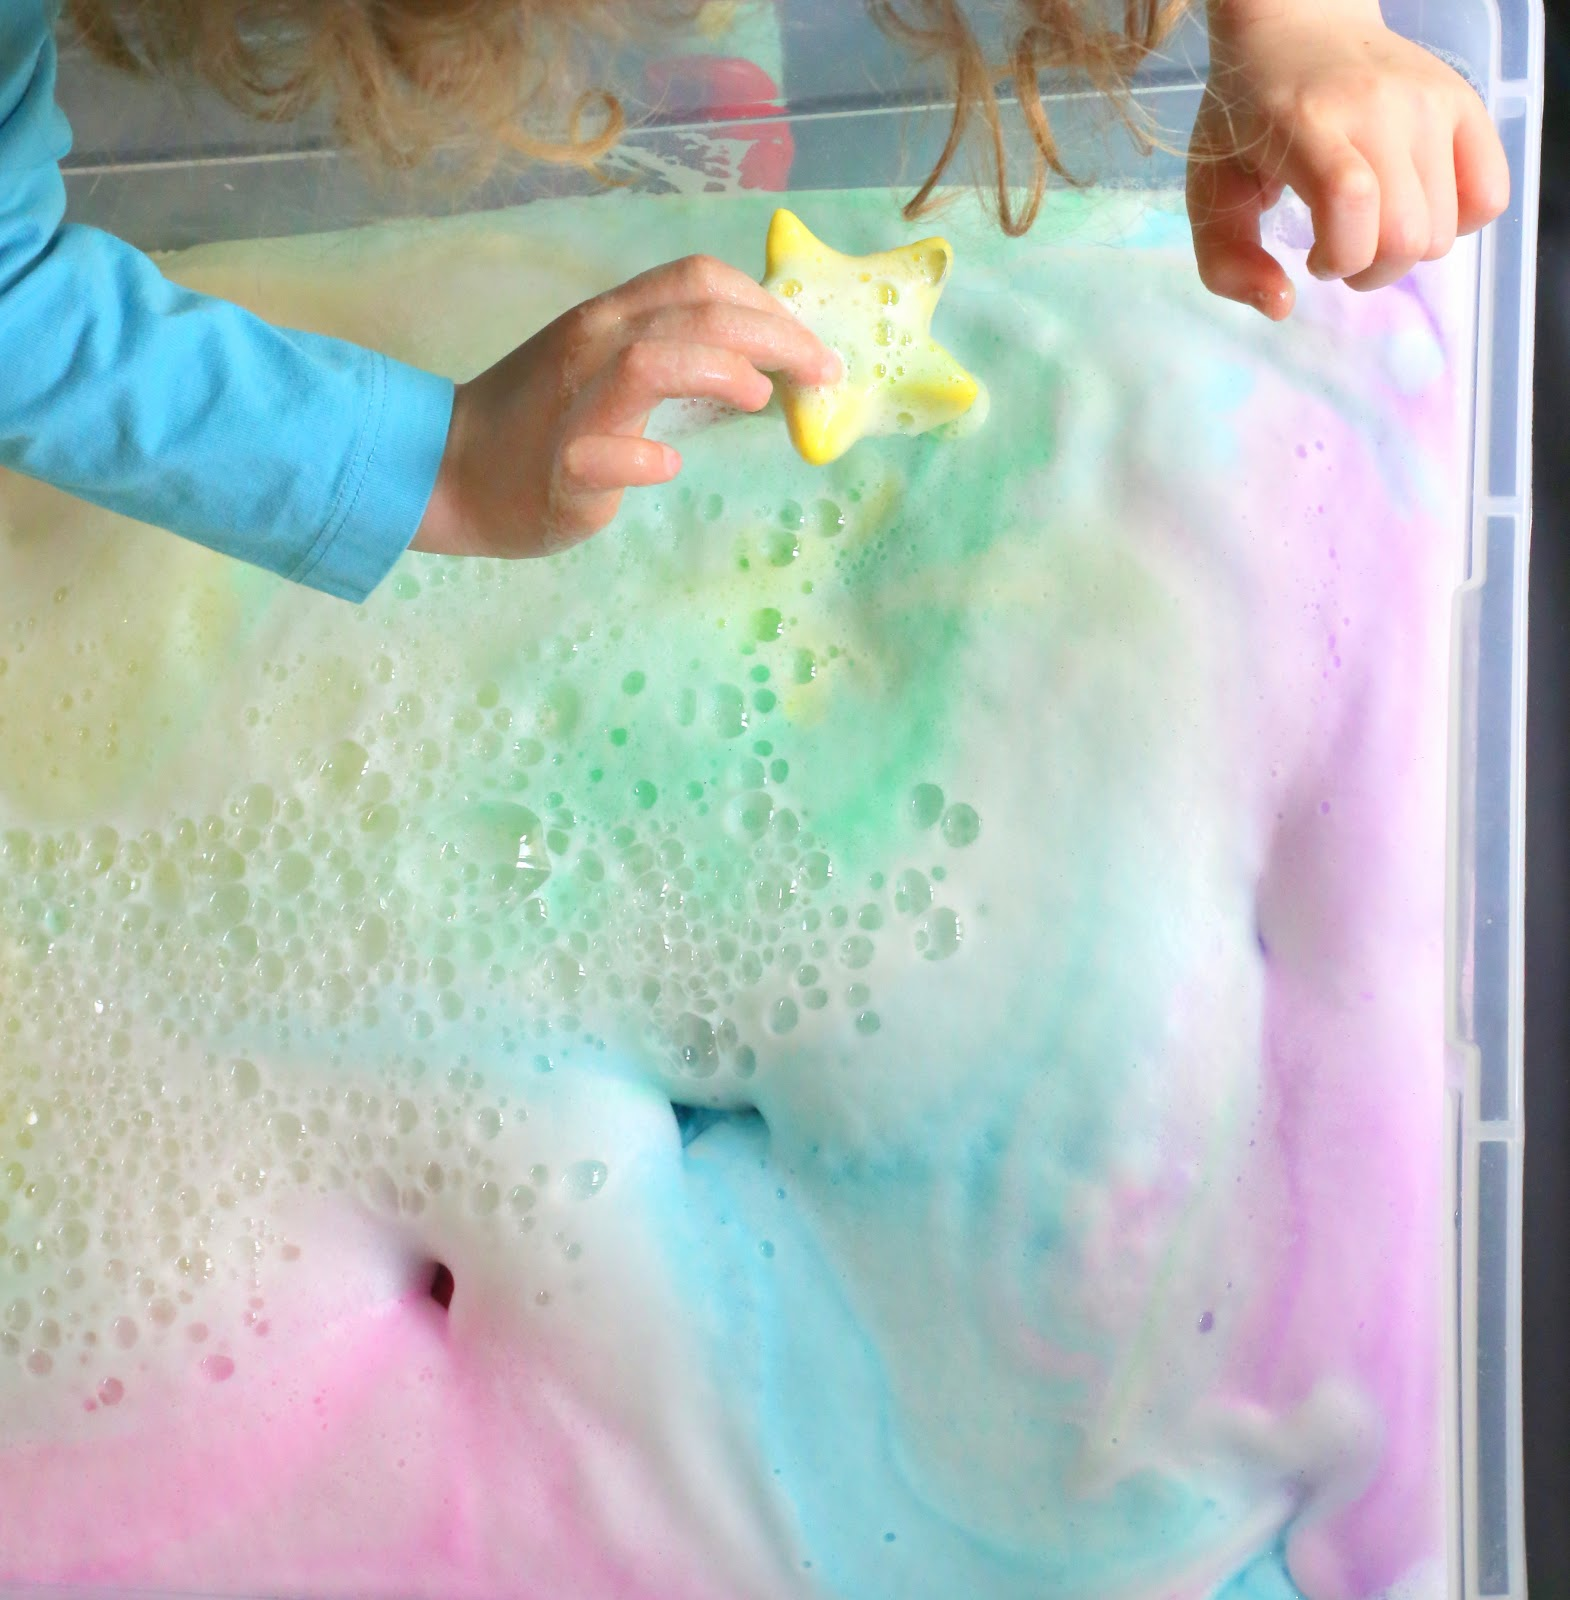
\includegraphics[scale=0.1]{1-IMG_4360.JPG}

{\tiny image © 2014 Asia Citro, reproduced with permission from \\
\url{http://www.funathomewithkids.com/2014/07/magic-foaming-treasure-stars.html}}
\end{figure}
\end{column}
\end{columns}

\end{frame}

\begin{frame}{Star-types}
A \emph{star-type} $\stps$ over $\TI$ is a nonempty subset
$\stps\subseteq\TI$ satisfying:
\begin{itemize}
  \item[\condstpx]\label{cond:stpx}
  If $\tpt, \tptp \in \stps$, then $\tpx\tpt = \tpx\tptp$.
  Denote $\tpx\tpt$ for any $\tpt \in \stps$ by $\tpp=\tpx\stps$.
  
  \item[\condstppy]\label{cond:stppy}
  If $\tppp \in \nb\TI\tpp$, then some $\tpt\in\stps$ has
  $\tpy\tpt = \tppp$.
  
  \item[\condstpky]\label{cond:stpky}
  If $\tpkp \in \nb\TI\tpp\cap\TK\TI$
  and if $\tpt,\tptp \in \stps$ have $\tpy\tpt = \tpy\tptp = \tpkp$,
  then $\tpt = \tptp$.
  
  \item[\condstpm]\label{cond:stpm}
  If $\sm \in \sms$, then some $\tpt\in\stps$ has $\sm(\xx,\yy) \in \tpTt$.
\end{itemize}
Then:
\begin{itemize}
  \item[\condstpkyu]\label{cond:stpkyu}
  If $\tpkp \in \nb\TI\tpp\cap\TK\TI$,
  then a unique $\tpt\in\stps$ has $\tpy\tpt = \tpk$.
\end{itemize}
\end{frame}

\begin{frame}{Certificates}
A \emph{certificate} $\Cert$ for $\TI$ is a nonempty set of star-types
satisfying:
\begin{itemize}
  \item[\condcertT]\label{cond:certT}
  If $\tpt\in\TI$, then some $\stps\in\Cert$ has $\tpt\in\stps$,
  that is there is a star-type containing each \twotype/.
  \item[\condcertk]\label{cond:certk}
  If $\tpk\in\TK\TI$ and if $\stps,\stpsp\in\Cert$
  have $\tpx\stps = \tpx\stpsp = \tpk$, then $\stps = \stpsp$.
\end{itemize}
Then:
\begin{itemize}
  \item[\condcertp]\label{cond:certp}
  If $\tpp \in \TP\TI$, then some $\stps\in\Cert$ has $\tpx\stps = \tpp$.
  \item[\condcertku]\label{cond:certku}
  If $\tpk \in \TK\TI$, then a unique $\stps\in\Cert$ has $\tpx\stps = \tpp$.
\end{itemize}
\end{frame}

\begin{frame}{Certificate Extraction}
Given a model $\StrA$ of $\TI$, $\Cert = \setbd{\stpIa\StrA\ea}{\ea\in\domA}$ is
a certificate, but it is \emph{too big}!
\pause

A star-type for every $\tpt\in\TI$ is sufficient!
\begin{itemize}
  \item For every $\tpt\in\TI$ choose $\eat\tpt,\ebt\tpt\in\domA$ such that
$\tpIab\StrA{\eat\tpt}{\ebt\tpt} = \tpt$
  \item $\Cert = \setbd{\stpIa\StrA{\eat\tpt}}{\tpt\in\TI}$ is a
  \emph{polynomial} certificate
\end{itemize}
\end{frame}

\begin{frame}{Certificate Expansion}
\begin{theorem}
Let $\Cert$ be a certificate for the type instance $\TI$ and let
$\pt\geq\card{\TI}$.
Then $\TI$ has a finite model in which every worker type is realized at least
$\pt$ times.
\end{theorem}
\end{frame}

\begin{frame}{Construction}
\begin{tikzpicture}
\draw[fill] (0,0) circle [radius=2pt];
\node[left] at (0,0) {$\ea_\tpk$};
\draw[dashed] (-1,-2.5) rectangle (1,1);
\node[below right] at (-1,1) {kings};
\node at (0,-1) {$\dots$};
\draw[dashed] (1,-2.5) rectangle (6,1);
\node[below right] at (1,1) {workers};

\draw[dashed] (1.5,0) rectangle (4.5,0.5);
\draw[fill] (1.75,0.25) circle [radius=2pt];
\node[right] at(1.75,0.25) {$\ea_{01}^\stps$};
\node at (3,0.25) {$\dots$};
\draw[fill] (3.5,0.25) circle [radius=2pt];
\node[right] at (3.5,0.25) {$\ea_{0t}^\stps$};

\draw[dashed] (2.5,-1) rectangle (5.5,-0.5);
\draw[fill] (2.75,-0.75) circle [radius=2pt];
\node[right] at(2.75,-0.75) {$\ea_{11}^\stps$};
\node at (4,-0.75) {$\dots$};
\draw[fill] (4.5,-0.75) circle [radius=2pt];
\node[right] at (4.5,-0.75) {$\ea_{1t}^\stps$};

\draw[dashed] (1.5,-2) rectangle (4.5,-1.5);
\draw[fill] (1.75,-1.75) circle [radius=2pt];
\node[right] at(1.75,-1.75) {$\ea_{21}^\stps$};
\node at (3,-1.75) {$\dots$};
\draw[fill] (3.5,-1.75) circle [radius=2pt];
\node[right] at (3.5,-1.75) {$\ea_{2t}^\stps$};

\draw (0,0) to (1.75,0.25);
\node[above] at (0.8,0.1) {$\tpt\in\stps$};
\draw (1.75,0.25) to (2.75,-0.75);
\draw (2.75,-0.75) to (1.75,-1.75);
\draw (1.75,-1.75) to (1.75,0.25);
\end{tikzpicture}
\begin{itemize}
  \item single element for each king
  \item $3$ blocks of $t$ elements for each worker star-type
  \item king--to--element determined by the star-type of the element
  \item worker--to--worker between consecutive blocks
  \item completion to a full structure
\end{itemize}
\end{frame}

\begin{frame}{Summary}
\begin{itemize}
  \item Type realizability for $\vFo2$ is in $\cNP$
  \item $\vFo2$ has the finite model property and its satisfiability problem is
  in $\cNExpTime$
\end{itemize}
\end{frame}

\section{Type Realizability with Equivalences in Refinement}
\begin{frame}{Refinement - Strategy}
\begin{itemize}
  \item Consider the two-variable logic with a single built-in equivalence symbol
  $\vFo2\Eea1\noag$
  \item Equivalence classes are structures for the \emph{simpler} $\vFo2$
  \item Exploit the previous result to ensure \emph{classes are ``consistent''} and
  figure out how to
  \emph{glue them together}
  \item Make sure the argument is suitable for induction to get to
  $\vFo2\Eea\sze\agrefine$
\end{itemize}
\end{frame}

\begin{frame}{Analogues}
\begin{align*}
  \vFo2 &\Longleftrightarrow \vFo2\Eea\sze\agrefine \\
  \text{models} &\Longleftrightarrow \text{nobly distinguished models} \\
  \text{elements} &\Longleftrightarrow \text{galaxies} \\
  \text{kings} &\Longleftrightarrow \text{noble galaxies} \\
  \text{workers} &\Longleftrightarrow \text{peasant galaxies} \\
  \text{star-types} &\Longleftrightarrow \text{locally consistent cosmic
  spectrums} \\
  \text{certificates} &\Longleftrightarrow \text{certificates}
\end{align*}
\end{frame}

\begin{frame}{Galaxies and Cosmos}
Let $\StrA$ be a $\vFo2\Eea1\noag$-structure for the type instance $\TI$.
\begin{itemize}
  \item classes of $\StrA$ are the \emph{galaxies} of $\StrA$
  \item $\StrA$ is \emph{the cosmos}
  \item $\tpt\in\TI$ is \emph{galactic} if $\se(\xx,\yy)\in\tpt$,
  $\TIg\subseteq\TI$
  \item otherwise $\tpt$ is \emph{cosmic}, $\TIc\subseteq\TI$
\end{itemize}
\end{frame}

\begin{frame}{Noble and Peasant Types}
\begin{itemize}
  \item
  $\tpn\in\TP\TI$ is \emph{noble} if no cosmic $\tpt$ has
  $\tpx\tpt = \tpy\tpt = \tpn$; the set of noble types is $\TN\TI$
  
  \item
  $\tpp\in\TP\TI$ is \emph{peasant} if it is not noble; the set of peasant types
  is $\TP\TI$
  
  \item
  kings are noble

  \item
  peasants are workers
  
  \item
  a galaxy is \emph{noble} if it realizes a noble type
  
  \item
  a galaxy is \emph{peasant} if it realizes only peasant types
\end{itemize}
\end{frame}

\begin{frame}{Example}
\begin{tikzpicture}
\draw[dashed] (-0.5,-1) rectangle (2.7,1);
\draw[fill] (0,0) circle[radius=2pt];
\node[right] at (0,0) {$\tpk$};
\draw[fill] (1,0.5) circle[radius=2pt];
\node[right] at (1,0.5) {$\tpn$};
\draw[fill] (1,-0.5) circle[radius=2pt];
\node[right] at (1,-0.5) {$\tpn$};
\draw[fill] (2,0) circle[radius=2pt];
\node[right] at (2,0) {$\tpp$};

\draw[dashed] (3,-1) rectangle (4,-0.2);
\draw[fill] (3.5,-0.6) circle[radius=2pt];
\node[right] at (3.5,-0.6) {$\tpp$};

\draw[dashed] (3,0.2) rectangle (4,1);
\draw[fill] (3.5,0.6) circle[radius=2pt];
\node[right] at (3.5,0.6) {$\tpp$};
\end{tikzpicture}

Noble galaxies may contain peasants!
\end{frame}

\begin{frame}{Noble Distinguishability}
\begin{itemize}
  \item A structure is \emph{nobly distinguished} if every noble galaxy realizes
  only noble types
  \pause
  \item Reduction: tag peasants in a noble galaxy with some noble type from that
  galaxy
  
  \begin{tikzpicture}
  \draw[dashed] (-0.5,-1) rectangle (2.7,1);
  \draw[fill] (0,0) circle[radius=2pt];
  \node[right] at (0,0) {$\tpk$};
  \draw[fill] (1,0.5) circle[radius=2pt];
  \node[right] at (1,0.5) {$\tpn$};
  \draw[fill] (1,-0.5) circle[radius=2pt];
  \node[right] at (1,-0.5) {$\tpn$};
  \draw[fill] (2,0) circle[radius=2pt];
  \node[right] at (2,0) {$\tpp_\tpn$};

  \draw[dashed] (3,-1) rectangle (4.5,-0.2);
  \draw[fill] (3.5,-0.6) circle[radius=2pt];
  \node[right] at (3.5,-0.6) {$\tpp_\bot$};

  \draw[dashed] (3,0.2) rectangle (4.5,1);
  \draw[fill] (3.5,0.6) circle[radius=2pt];
  \node[right] at (3.5,0.6) {$\tpp_\bot$};
  \end{tikzpicture}
\end{itemize}
\end{frame}

\begin{frame}{Cosmic Spectrums}
\begin{itemize}
  \item Let $\StrA$ be a nobly distinguished model for $\TI$ having at least $2$
  galaxies
  \item The cosmic spectrum of a galaxy $\galX\subset\domA$ is
   \[
   \cspIX\StrA\galX = (\cii\csps,\cie\csps,\cei\csps,\cee\csps)
   \]
\begin{tikzpicture}
\draw[dashed] (-1,-1) rectangle (1,1);
\node[above right] at (-1,1) {$\galX$};
\draw[fill] (-0.5,0.5) circle[radius=2pt];
\draw[fill] (0.5,0.5) circle[radius=2pt];
\draw (-0.5,0.5) to (0.5,0.5);
\node[above] at (0.2,0.4) {$\tpt\in\cii\csps$};
\draw[fill] (0.7,0) circle[radius=2pt];
\draw[fill] (2.1,0) circle[radius=2pt];
\draw (0.7,0) to (2.1,0);
\node[above] at (1.7,-0.1) {$\tpt\in\cie\csps$};
\node[below] at (1.8,0.1) {$\inv\tpt\in\cie\csps$};
\draw[fill] (2.1,0.8) circle[radius=2pt];
\draw[fill] (3.1,0.8) circle[radius=2pt];
\draw (2.1,0.8) to (3.1,0.8);
\node[above] at (2.8,0.7) {$\tpt\in\cee\csps$};
\end{tikzpicture}
\end{itemize}
\end{frame}

\begin{frame}{Cosmic Spectrums}
A cosmic spectrum $\csps=(\cii\csps,\cie\csps,\cei\csps,\cee\csps)$ over $\TI$
is a tuple satisfying:
\begin{itemize}
  \item[\condcspII]\label{cond:cspII}
  The set of \emph{internal types} $\cii\csps \subseteq \TIg$ is a set of
  galactic types that is closed under inversion.
  
  \item[\condcspIE]\label{cond:cspIE}
  The set of \emph{boundary types} $\cie\csps \subseteq \TIc$ is a nonempty set
  of cosmic types.
  
  \item[\condcspEI]\label{cond:cspEI}
  The set of \emph{inverted boundary types} is:
  $\cei\csps = \setbd{\inv\tpt}{\tpt\in\cie\csps}$.
  
  \item[\condcspEE]\label{cond:cspEE}
  The set of \emph{external types} $\cee\csps \subseteq \TI$ is a set of
  \twotypes/ that is closed under inversion.

  \item[\condcspT]\label{cond:cspT}
  We require that
  $\TI = \cii\csps \cup \cie\csps \cup \cei\csps \cup \cee\csps$.

  \item[\condcspNP]\label{cond:cspNP}
  The (nonempty) set $\Tpx\csps = (\tpx\restriction{\cie\csps})$ is
  the set of \emph{internal \onetypes/} of~$\csps$.
  We require that $\Tpx\csps \subseteq \TN\TI$ or $\Tpx\csps \subseteq \TPs\TI$.
\end{itemize}
\end{frame}

\begin{frame}{Locally consistent cosmic spectrums}
\begin{itemize}
\item The \emph{spectral type instance} $\TIs$ of the
$\vFo2\Eea\sze\agrefine$-cosmic spectrum $\csps$ is $\TIs = \dii\TIs \cup \die\TIs \cup \dei\TIs \cup \dee\TIs$,
where $\TIs_{\mathcal{X}{\mathcal{Y}}} =
\setbd{\tpt_{\mathcal{X}{\mathcal{Y}}}}{\tpt\in\csps^{\mathcal{X}\mathcal{Y}}}$,
where $\tpt_{\mathcal{X}{\mathcal{Y}}}$ works by ``removing $\se$ and tagging
the ends with a new predicate symbol $\si$''.

\item $\csps$ is \emph{locally consistent} if $\TIs$ is realizable over
\emph{the simpler} $\vFo2\Eea{(\sze-1)}\agrefine$

\begin{tikzpicture}
\node[above right] at (-1,1) {$\StrA : \vFo2\Eea\sze\agrefine$};
\draw (-1,-1) rectangle (2,1);
\draw[dashed] (-0.8,-0.8) rectangle (0.5,0.8);
\node[below right] at (-0.8,0.8) {$\galX$};
\draw[fill] (-0.2,0) circle[radius=2pt];
\node[right] at (-0.2,0) {$\tpp$};
\draw[fill] (1,0) circle[radius=2pt];
\node[right] at (1,0) {$\rho$};

\node at (3,0) {$\implies$};

\draw (4,-1) rectangle (9,1);
\node[above right] at (4,1) {$\StrAp : \vFo2\Eea{(\sze-1)}\agrefine$};
\draw[dashed] (4.2,-0.8) rectangle (6.3,0.8);
\node[below right] at (4.2,0.8) {$\si$};
\draw[fill] (4.5,0) circle[radius=2pt];
\node[right] at (4.5,0) {$\tpp^{-\se}+\si$};
\node[below right] at (6.3,0.8) {$\lnot\si$};
\draw[fill] (6.6,0) circle[radius=2pt];
\node[right] at (6.6,0) {$\tpr^{-\se}+(\lnot\si)$};
\end{tikzpicture}
\end{itemize}
\end{frame}

\begin{frame}{Certificates}
A \emph{certificate} $\Cert$ for the type instance~$\TI$ is a nonempty set of
locally consistent cosmic spectrums satisfying:
\begin{itemize}
  \item[\condcertTc]\label{cond:certTc}
  If $\tpt\in\TIc$ then some $\csps\in\Cert$ has $\tpt\in\cie\csps$.
  \item[\condcertTg]\label{cond:certTg}
  If $\tpt\in\TIg$ then some $\csps\in\Cert$ has $\tpt\in\cii\csps$.
  \item[\condcertn]\label{cond:certn}
  If $\tpn\in\TN\TI$ and $\csps,\cspsp\in\Cert$ have $\tpn\in\Tpx\csps$ and
  $\tpn\in\Tpx\cspsp$, then $\cspsp = \csps$.
\end{itemize}
\end{frame}

\begin{frame}{Certificate Expansion}
\begin{theorem}
Let $\Cert$ be a certificate for the type instance $\TI$ over the
$\vFo2\Eea\sze\agrefine$-classified signature $\ClSig\Sigma\sms$.
Then $\TI$ has a finite model in which each worker type is realized at least
$\pt$ times.
\end{theorem}
\begin{itemize}
  \item Type realizability for $\vFo2\Eea\sze\agrefine$ is in
  $\cNP$
  \item Satisfiability for $\vFo2\Eea\sze\agrefine$ is in
  $\cNExpTime$
\end{itemize}
\end{frame}
\end{document}